\documentclass[a5paper]{article}
\usepackage[a5paper, top=8mm, bottom=8mm, left=8mm, right=8mm]{geometry}

\usepackage{polyglossia}
\setdefaultlanguage[babelshorthands=true]{russian}

\usepackage{fontspec}
\setmainfont{FreeSerif}
\newfontfamily{\russianfonttt}[Scale=0.7]{DejaVuSansMono}

\usepackage[font=scriptsize]{caption}

\usepackage{amsmath}
\usepackage{amssymb,amsfonts,textcomp}
\usepackage{color}
\usepackage{array}
\usepackage{hhline}
\usepackage{cite}
\usepackage{color}

\usepackage[hang,multiple]{footmisc}
\renewcommand{\footnotelayout}{\raggedright}

\PassOptionsToPackage{hyphens}{url}\usepackage[xetex,linktocpage=true,plainpages=false,pdfpagelabels=false]{hyperref}
\hypersetup{colorlinks=true, linkcolor=blue, citecolor=blue, filecolor=blue, urlcolor=blue, pdftitle=1, pdfauthor=, pdfsubject=, pdfkeywords=}

\usepackage{tabu}

\usepackage{graphicx}
\usepackage{indentfirst}
\usepackage{multirow}
\usepackage{subfig}
\usepackage{footnote}
\usepackage{minted}

\sloppy
\pagestyle{plain}

\title{Базы данных}
\author{Юрий Литвинов\\\small{yurii.litvinov@gmail.com}}

\date{13.02.2019г}

\begin{document}

\maketitle
\thispagestyle{empty}

\section{Введение}

Без работы с базами данных не обходится ни одно веб-приложение и вообще ни одно приложение, которому надо что-то долго хранить и быстро получать доступ к данным. В принципе, люди долгое время прекрасно обходились обычными файлами, да и для задач типа хранения настроек приложения обычные файлы конфигурации вполне подходят. Но данные часто имеют сложную структуру, к ним приходится выполнять кучу разных видов запросов, к тому же данных, если они заводятся в вашем приложении, быстро становится очень много и они перестают помещаться в оперативке.

Кстати, есть базы данных, а есть системы управления базами данных. БД --- это, собственно, данные вместе с их структурой, СУБД --- это программа, которая предоставляет к этим данным доступ и позволяет их редактировать (или их структуру). СУБД бывают концептуально разные, каждый подход имеет свои достоинства и недостатки:

\begin{itemize}
	\item Реляционные --- до сих пор самый популярный вид СУБД, использующий реляционную алгебру (\url{https://en.wikipedia.org/wiki/Relational_algebra}) для представления данных и операций над ними. Данные в реляционной модели представляются в виде \textit{кортежей} значений разных типов, объединённых в \textit{отношения} --- самые настоящие алгебраические отношения и кортежи, в простонародье называемые таблицами и строками. На отношениях определены алгебраические операции, которые принимают отношения и возвращают отношения, определены совершенно формально и их свойства хорошо изучены. Эти алгебраические операции выражаются операторами языка SQL, который достаточно прост, чтобы им мог пользоваться любой школьник, несмотря на то, что внутри происходит кошмарная алгебраическая наука. Операции достаточно выразительны, чтобы с данными можно было делать практически всё, что угодно, и при этом достаточно декларативны, чтобы СУБД могла сама решать, как исполнять запрос, оптимизируя его зачастую в тысячи раз по сравнению с наивной реализацией.
	\item Объектно-ориентированные --- хранят по сути сериализованные объекты и позволяют исполнять запросы в духе ``найти объект по шаблону''. Значительно менее выразительный язык запросов компенсируется удобством использования из объектно-ориентированных программ --- результатом операции становится не какой-то невнятный набор кортежей, которые ещё надо как-то загрузить в объектно-ориентированную программу, а самый настоящий объект, будто мы его хранили в памяти. К тому же, такие базы, как правило, проще в конфигурировании и использовании, так что очень популярны сейчас для хранения небольших объёмов данных или данных, не предполагающих сложных запросов.
	\item Иерархические --- СУБД, хранящие данные в виде дерева. Самый типичный нынче пример таких штук --- базы, хранящие данные в XML-документах. Для запросов там используется язык XQuery, работающий с выражениями на языке XPath. Для иерархических по своей природе данных такие штуки незаменимы.
	\item Другие --- например, дедуктивные базы данных, которые вообще не хранят данные, они хранят некоторый набор фактов и правила, по которым могут быть выведены остальные факты (например, см. \url{https://en.wikipedia.org/wiki/Datalog}). 
\end{itemize}

Наиболее популярны сейчас всё-таки реляционные и объектно-ориентированные базы данных, поэтому часто приходится решать, какую же из этих моделей использовать. Так что рассмотрим соображения, могущие повлиять на решение:

\begin{itemize}
	\item Реляционные
	\begin{itemize}
		\item Минусы --- сложность интеграции с объектно-ориентированным кодом. Реляционная модель данных концептуально построена по принципу ``сущность-связь'', где сущность --- это штука, у которой есть имя и атрибуты, могущие иметь значения, а связь --- это ссылка из одной сущности на другую. Это очень похоже на объекты и отношения между ними, так что, казалось бы, никаких пробелм быть не должно, но нет: сущности не могут наследоваться, друг от друга, например. Чтобы хранить в реляционной базе объекты двух разных классов, наследующихся от общего предка, потребуется либо две таблицы с атрибутами, куда раскопипащены атрибуты предка, либо три таблицы --- для предка и двух потомков, и явные связи между потомками и предком. При загрузке и сохранении таких ``объектов'' фактически приходится реализовывать наследование вручную. Ещё реляционные базы не могут в отношение ``многие ко многим'', потому что связь там --- это просто ссылка на строку в другой таблице, она может быть только одной. Для решения этой проблемы заводят вспомогательные ``таблицы-развязки'', хранящие в себе только набор связей.
		\item Плюсы --- выразительный язык запросов, который даже со всякими там таблицами-развязками позволяет выбрать именно те данные, что нужны, и представить их в более-менее удобном виде. Кроме того, запросы выполняются, как правило, очень эффективно, грамотный проектировщик схемы БД может сделать так, чтобы выборка из сотен гигабайт данных занимала всего доли секунды. Впрочем, неудачная схема БД может испортить скорость работы всего приложения очень серьёзно.
	\end{itemize}
\end{itemize}

\section{Реляционная модель данных}

Рассмотрим подробнее реляционную модель (без алгебраических деталей). Данные там хранятся в виде отношений, которые удобнее всего себе представлять как таблицы, как на рисунке~\ref{image:table} из Википедии.

\begin{figure}
	\begin{center}
		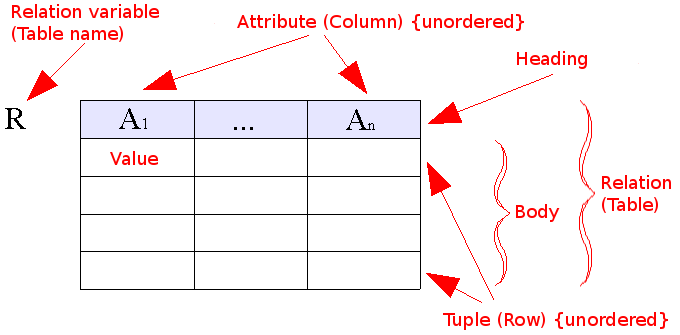
\includegraphics[width=0.7\textwidth]{relationalModel.png}
	\end{center}
	\caption{Отношение.}
	\label{image:table}
\end{figure}

У отношения есть имя (имя таблицы), у него есть колонки с именами и типами, и строчки, состоящие из, собственно, данных, лежащих в таблице. Пример таблицы с данными представлен в~\ref{table:tableWithData}.

\begin{figure}
	\begin{center}
		\begin{tabu} {| X[0.9 l p] | X[1 l p] | X[1 l p] | X[1 l p] |}
			\tabucline-
			CustomerID       & TaxID        & Name       & Address           \\
			\tabucline-
			\everyrow{\tabucline-}
			1234567890       & 555-5512222  & Munmun     & 323 Broadway      \\
			2223344556       & 555-5523232  & Wile E.    & 1200 Main Street  \\
			3334445563       & 555-5533323  & Ekta       & 871 1st Street    \\
			423242432        & 555-5325523  & E.F. Codd  & 123 It Way        \\
		\end{tabu}
	\end{center}
	\caption{Таблица с данными.}
	\label{table:tableWithData}
\end{figure}

\subsection{Ключи}

Если бы все данные, которые нужны программе, можно было хранить в одной таблице, то никакая реляционная алгебра была бы не нужна. Интереснее становится, когда данные имеют сложную структуру, требующую нескольких связанных таблиц. Например, список городов и список улиц, где каждая улица привязана к конкретному городу (рис.~\ref{table:citiesStreets})

\begin{figure}
	\begin{center}
		CITY
		\begin{tabu} {| X[0.2 l p] | X[1 l p] |}
			\tabucline-
			ID      & Name \\
			\tabucline-
			\everyrow{\tabucline-}
			1       & Москва \\
			2       & Санкт-Петербург \\
			3       & Владивосток \\
		\end{tabu}
		\vspace{3mm}
		STREET
		\begin{tabu} {| X[0.2 l p] | X[1 l p] | X[0.7 l p] |}
			\tabucline-
			ID       & Name             & ID\_CITY \\
			\tabucline-
			\everyrow{\tabucline-}
			181      & Малая Бронная    & 1 \\
			182      & Тверской Бульвар & 1 \\
			183      & Невский проспект & 2 \\
			184      & Пушкинская       & 2 \\
			185      & Светланская      & 3 \\
			186      & Пушкинская       & 3 \\
		\end{tabu}
	\end{center}
	\caption{Таблицы с городами и улицами.}
	\label{table:citiesStreets}
\end{figure}

В принципе, всё можно было сложить и в одну таблицу (хранить в STREET просто названия городов), но, во-первых, это дупликация данных, во-вторых, города могут понадобиться кому-то ещё.

Как в базах данных работают ссылки на другие таблицы --- очень просто, на самом деле. Есть понятие ``ключ'', набор столбцов, уникально идентифицирующих любой кортеж в таблице. Первичный ключ --- это уникальный идентификатор в таблице с нашими данными, внешний ключ --- это уникальный идентификатор наших данных, сохранённый в какой-то другой таблице. В примере~\ref{table:citiesStreets} первичным ключом в таблице CITY был столбец ID, в таблице STREET тоже есть первичный ключ (и тоже ID), но есть и внешний ключ --- столбец ID\_CITY, где просто записаны первичные ключи городов, которым принадлежат улицы. 

Может показаться, что первичный ключ --- это всегда число, что-то вроде номера ячейки памяти, но нет, они бывают разные. Бывают естественные первичные ключи --- идентификаторы, присущие самим данным, например, номер паспорта или номер зачётки. Они уникальны по самой своей природе, поэтому вполне подходят в качестве первичных ключей. Бывают даже составные ключи --- ключи, состоящие из нескольких колонок. Например, название не идентифицирует город однозначно, но название страны, название региона плюс название города --- вполне себе уникальный идентификатор. Тогда в качестве внешнего ключа приходится использовать все значения, входящие в составной ключ.

Суррогатными ключами называются ключи, которых нет в предметной области, и их пришлось специально придумать, чтобы однозначно идентифицировать объекты (например, ID из~\ref{table:citiesStreets}). Они используюся чаще, чем естественные, потому что они заведомо уникальны --- например, MAC-адрес было бы разумно использовать как естественный ключ, но только до тех пор, пока нам не попадутся две сетевые карты с одинаковым MAC-адресом, который должен быть глобально уникальным. Кроме того, они компактнее, чем большинство естественных ключей. Но не очень хорошо работают в сценариях, когда требуется использовать данные из двух разных баз данных, так что естественные ключи всё-таки бывают полезны.

\subsection{Ограничения}

Базе данных можно сказать, что колонка --- это первичный ключ, тогда она будет сама проверять его уникальность (и даже генерить, если попросить). Это делается с помощью \textit{ограничений} --- свойств колонок в схеме БД. Первичные ключи описываются как ограничение PRIMARY KEY (чуть попозже будет понятно, куда это писать). Бывает ещё ограничение FOREIGN KEY, заставляющее СУБД проверять, что такой ключ действительно есть в таблице, на которую ссылается внешний ключ (сам ключ не ссылается, это просто значение, но в самом ограничении можно указать, о какой таблице идёт речь). Отметим, что кортеж, на который ссылается какой-то из внешних ключей, нельзя удалить (без \textit{каскадного удаления}, по крайней мере, когда удаляется и кортеж, и все кортежи, которые на него ссылаются, и все кортежи, которые ссылаются на них, и т.д.).

Есть ещё ограничение NOT NULL, заставляющее атрибут всегда иметь значение (по умолчанию значение любого типа может быть NULL, что означает отсутствие значения), и UNIQUE, что заставляет значение быть уникальным в своей колонке. Попытка вставить данные, которые нарушают уникальность, будет отклонена СУБД.

\section{SQL}

Теперь, собственно, про то, как работать с реляционными данными. Для этого чаще всего используется язык SQL (Structured Query Language). Он был специально спроектирован так, чтобы быть максимально простым и похожим на разговорный английский. 

\subsection{SELECT}

Самый известный, пожалуй, оператор SQL --- это SELECT (да, в SQL ключевые слова по традиции пишут капсом, хотя сам язык регистронезависимый, как Паскаль). SELECT позволяет выбрать данные по некоторому критерию из некоторой таблицы или некоторого набора таблиц, получив новую таблицу (это алгебраический оператор, мы хотим замкнутость, так что да, результат SELECT --- таблица). Несколько примеров из Википедии приведены на рис.~\ref{image:select}, подробное описание можно посмотреть на \url{https://www.w3schools.com/sql/sql_select.asp} (учтите, что почти каждая СУБД имеет свой диалект SQL, так что синтаксис и возможности могут немного различаться, но для часто используемых случаев всё будет работать везде).

\begin{figure}
	\begin{center}
		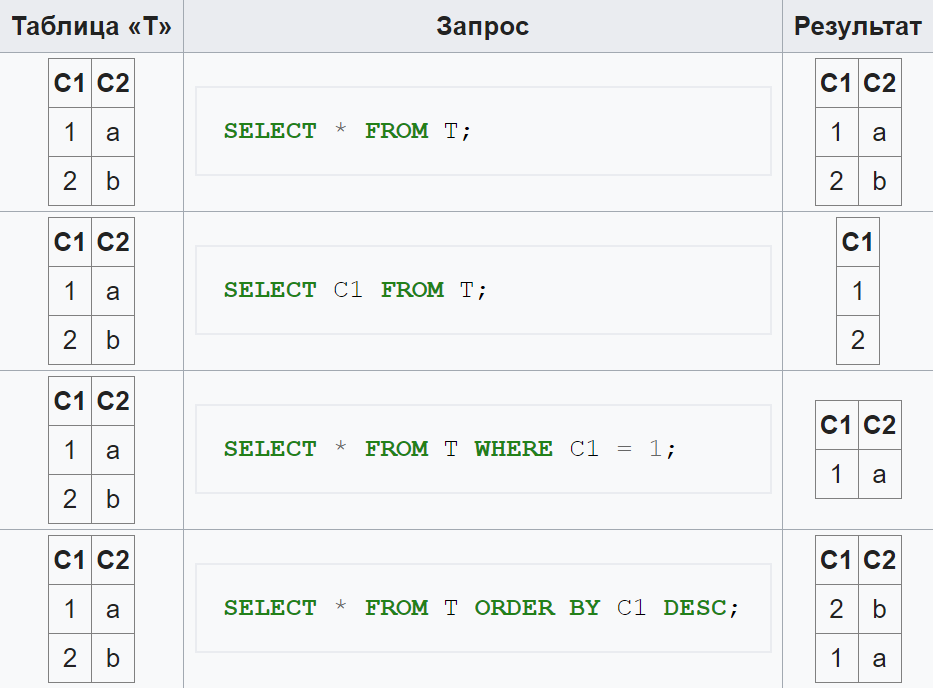
\includegraphics[width=0.6\textwidth]{select.png}
	\end{center}
	\caption{Оператор SELECT.}
	\label{image:select}
\end{figure}

Самое интересное тут, пожалуй, WHERE --- часть с предикатом, который определяет, какие кортежи попадут в результирующее отношение. Именно благодаря WHERE можно выбирать только те данные, которые нужны, и не грузить в оперативку все сотни гигов данных из базы.

SELECT поддерживает вложенные запросы и агрегатные функции. Например, 

\begin{minted}{sql}
SELECT isbn,
       title,
       price
FROM Book
WHERE price < (SELECT AVG(price) FROM Book)
ORDER BY title;
\end{minted}

Этот запрос выбирает книги с ценой, меньшей средней, и сортирует их по названию. AVG --- агрегатная функция, принимает имя колонки и возвращает среднее значение числовых данных в этой колонке. Обратите внимание на то, что все функции вызываются как запросы к БД, через SELECT.

\subsection{INNER JOIN}

Самая, пожалуй, важная функциональность SELECT-а связана с возможностью получать данные из нескольких таблиц сразу, объединяя результаты запроса в новую таблицу. Например, рассмотрим таблицы с рисунка~\ref{table:citiesPeople}.

\begin{figure}
	\begin{center}
		\begin{tabular}{c c}
			CITY & STREET \\
			\begin{tabu} to 0.3\textwidth {| X[0.2 l p] | X[1 l p] |}
				\tabucline-
				ID      & Name \\
				\tabucline-
				\everyrow{\tabucline-}
				1       & Москва \\
				2       & Санкт-Петербург \\
				3       & Владивосток \\
			\end{tabu}
			&
			\begin{tabu} to 0.5\textwidth {| X[0.5 l p] | X[1 l p] |}
				\tabucline-
				Name             & CITY\_ID \\
				\tabucline-
				\everyrow{\tabucline-}
				Андрей      & 1 \\
				Леонид      & 1 \\
				Сергей      & 2 \\
				Григорий    & 4 \\
			\end{tabu}
		\end{tabular}
	\end{center}
	\caption{Таблицы с городами и улицами.}
	\label{table:citiesPeople}
\end{figure}

Вот так можно получить названия городов, в которых живут люди:

\begin{minted}{sql}
SELECT * FROM Person INNER JOIN City ON Person.CityId = City.CityId
\end{minted}

То есть SELECT берёт данные из Person и City, дальше объединяет два кортежа, таких что их CityId совпадают, в один кортеж, и всё, что получилось, складывает в результирующую таблицу. Результат можно посмотреть в~\ref{table:citiesPeopleResult}.

\begin{figure}
	\begin{center}
		\begin{tabu}{| X[1 l p] | X[1 l p] | X[1 l p] | X[1 l p]  |}
			\tabucline-
			Person.Name  & Person.CityId  & City.Id  & City.Name       \\
			\tabucline-
			\everyrow{\tabucline-}
			Андрей       & 1              & 1        & Москва          \\
			Леонид       & 1              & 1        & Москва          \\
			Сергей       & 2              & 2        & Санкт-Петербург \\
		\end{tabu}
	\end{center}
	\caption{Результат запроса.}
	\label{table:citiesPeople}
\end{figure}

Эта конструкция настолько часто используется, что работает и вот так:

\begin{minted}{sql}
SELECT * FROM Person, City WHERE Person.CityId = City.CityId
\end{minted}

\subsection{OUTER JOIN}

INNER JOIN не добавляет в результат данные, которым не нашлось ``пары'' в хотя бы одной из таблиц (это логично, с чего бы, для них ведь условие в WHERE не выполняется). Иногда всё же надо получить результат, включающий в себя все данные, включая те, для которых не нашлось соответствия. Это делает OUTER JOIN:

\begin{minted}{sql}
SELECT * FROM Person LEFT OUTER JOIN City ON Person.CityId = City.CityId
\end{minted}

Результат теперь получится таким:

\begin{center}
	\begin{tabu}{| X[1 l p] | X[1 l p] | X[1 l p] | X[1 l p] |}
		\tabucline-
		Person.Name  & Person.CityId  & City.Id  & City.Name       \\
		\tabucline-
		\everyrow{\tabucline-}
		Андрей       & 1              & 1        & Москва          \\
		Леонид       & 1              & 1        & Москва          \\
		Сергей       & 2              & 2        & Санкт-Петербург \\
		Григорий     & 4              & NULL     & NULL            \\
	\end{tabu}
\end{center}

Обратите внимание, что OUTER JOIN не симметричен --- сейчас в выдачу попал Григорий, но если бы мы записали таблицы в другом порядке, в выдачу бы попал Владивосток.

\subsection{CROSS JOIN}

Ещё бывает CROSS JOIN --- это на самом деле просто SELECT по нескольким таблицам без ON или WHERE. Что он делает, несложно догадаться --- просто объединяет всё со всем, строя фактически декартово произведение кортежей. Например, если написать

\begin{minted}{sql}
SELECT * FROM Person, City
\end{minted}

получится

\begin{center}
	\begin{tabu}{| X[1 l p] | X[1 l p] | X[1 l p] | X[1 l p] |}
		\tabucline-
		Person.Name  & Person.CityId  & City.Id  & City.Name       \\
		\tabucline-
		\everyrow{\tabucline-}
		Андрей       & 1              & 1        & Москва          \\
		Андрей       & 1              & 2        & Санкт-Петербург \\
		Андрей       & 1              & 3        & Владивосток     \\
		Леонид       & 1              & 1        & Москва          \\
		Леонид       & 1              & 2        & Санкт-Петербург \\
		Леонид       & 1              & 3        & Владивосток     \\
		Сергей       & 2              & 1        & Москва          \\
		Сергей       & 2              & 2        & Санкт-Петербург \\
		Сергей       & 2              & 3        & Владивосток     \\
		Григорий     & 4              & 1        & Москва          \\
		Григорий     & 4              & 2        & Санкт-Петербург \\
		Григорий     & 4              & 3        & Владивосток     \\
	\end{tabu}
\end{center}

Как правило, такой запрос  получается случайно, при этом СУБД честно пытается его выполнить, строит огромное декартово произведение и падает из-за недостатка оперативки.

\subsection{Таблицы-развязки}

Теперь, наконец, можно рассказать, как в реляционной можели реализуется отношение ``многие-ко-многим''. Например, мы хотим хранить данные о научных статьях и их авторах, но у статьи может быть много авторов и у автора может быть много статей. Тогда нам потребуется ещё одна таблица, которая будет хранить соответствие автора и статьи. Например,

\begin{center}
	\begin{tabular}{c c c}
		Author & AuthorArticle & Article \\
		\begin{tabu} to 0.25\textwidth {| X[0.2 l p] | X[1 l p] |}
			\tabucline-
			ID      & Name \\
			\tabucline-
			\everyrow{\tabucline-}
			1       & Терехов \\
			2       & Брыксин \\
			3       & Литвинов \\
		\end{tabu}
		&
		\begin{tabu} to 0.25\textwidth {| X[1 l p] | X[1 l p] |}
			\tabucline-
			AuthorId             & ArticleId \\
			\tabucline-
			\everyrow{\tabucline-}
			1   & 1 \\
			1   & 2 \\
			2   & 1 \\
			2   & 3 \\
			3   & 1 \\
			3   & 3 \\
		\end{tabu}
		&
		\begin{tabu} to 0.45\textwidth {| X[0.1 l p] | X[1 l p] |}
			\tabucline-
			ID      & Title \\
			\tabucline-
			\everyrow{\tabucline-}
			1       & Архитектура среды визуального моделирования QReal \\
			2       & Технология программирования \\
			3       & Среда визуального программирования роботов QReal:Robots \\
		\end{tabu}
	\end{tabular}
\end{center}

Наличие такой таблицы-развязки позволяет использовать её в WHERE (или ON) при выполнении SELECT-а. Например, как узнать все статьи Андрея Николаевича Терехова, зарегистрированные в нашей базе:

\begin{minted}{sql}
SELECT Article.Title FROM Author, AuthorArticle, Article 
    WHERE Author.Id = AuthorArticle.AuthorId 
        AND AuthorArticle.ArticleId = Article.Id 
        AND Author.Name = 'Терехов'
\end{minted}

Или как найти всех авторов статьи ``Среда визуального программирования роботов QReal:Robots'':

\begin{minted}{sql}
SELECT Author.Name FROM Author, AuthorArticle, Article 
    WHERE Author.Id = AuthorArticle.AuthorId 
        AND AuthorArticle.ArticleId = Article.Id 
        AND Article.Title = 'Среда визуального программирования роботов QReal:Robots'
\end{minted}

\subsection{INSERT, UPDATE, DELETE}

Вставлять новые данные в базу можно с помощью оператора INSERT. Выглядит это примерно так:

\begin{minted}{sql}
INSERT INTO City(Name) VALUES ('Казань');
\end{minted}

Указывается имя таблицы, в скобках имена столбцов, которые мы хотим задать, затем после VALUES значения, которые нужно сохранить в новый кортеж. Если не указали столбец, который может автогенерироваться (например, суррогатный первичный ключ), СУБД подберёт для него значение сама. Иначе вставятся NULLы. Если NULLы нельзя, запрос будет отклонён.

Поменять уже существующие данные можно с помощью оператора UPDATE:

\begin{minted}{sql}
UPDATE persons SET
        street = 'Nissestien 67',
        city = 'Sandnes',
    WHERE lastname = 'Tjessem' AND firstname = 'Jakob';
\end{minted}

Забыть указать WHERE --- любимая ошибка начинающих пользователей баз данных. Тогда новое значение будет присвоено всем столбцам в таблице вообще.

Ну и удаление делается через оператор DELETE:

\begin{minted}{sql}
DELETE ab, b
    FROM Authors AS a, AuthorArticle AS ab, Articles AS b
    WHERE a.AuthID = ab.AuthID AND ab.ArticleID = b.ArticleID
        AND AuthorLastName = 'Henry';
\end{minted}

Такой запрос удалит все статьи, написанные неким Henry из базы данных, вместе с записями в таблице-развязке.

\subsection{Работа с метаинформацией}

Схема базы данных (то, какие таблицы есть в базе, какие и какого типа колонки, ограничения) задаётся тоже на самом деле на SQL. Для этого есть несколько операторов.

Создание таблицы --- это CREATE TABLE:

\begin{minted}{sql}
CREATE TABLE Students (
    Code INTEGER NOT NULL,
    Name NCHAR(30) NOT NULL,
    Address NVARCHAR(50),
    Mark DECIMAL);
\end{minted}

Здесь мы создаём таблицу Students, у которой есть поля Code типа INTEGER, Name типа NCHAR(30) (Юникодная строка фиксированной длины 30), Address типа NVARCHAR(50) (Юникодная строка максимальной длины 50, но могущей быть меньше), Mark типа DECIMAL. Кроме того, тут же указано, что Code и Name не могут быть NULLами.

Удаление таблицы:

\begin{minted}{sql}
DROP TABLE Students;
\end{minted}

Тут всё должно быть и так понятно, на xkcd был даже комикс по этому поводу:

\begin{center}
	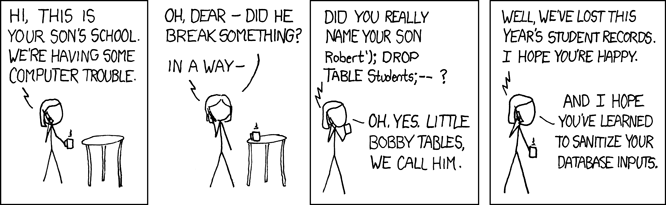
\includegraphics[width=0.6\textwidth]{bobbyTables.png}
\end{center}

Точка с запятой в SQL разделяет операторы, с ``--'' начинается комментарий (чтобы продолжение команды не вызвало синтаксическую ошибку и DROP TABLE таки отработала). Типичный пример SQL-инъекции.

Модификация таблицы:

\begin{minted}{sql}
ALTER TABLE Students ADD email VARCHAR(MAX);
ALTER TABLE Students DROP COLUMN email;
ALTER TABLE Students ADD PRIMARY KEY (Code);
\end{minted}

Тут мы добавили новый столбец, удалили столбец, добавили ограничение, что Code является первичным ключём (следовательно, должен быть уникальным).

\section{Демонстрация}

Теперь предлагается попробовать поработать с живой СУБД, пока на уровне SQL. Это, кстати, хороший способ проверить адекватность схемы БД и правильность SQL-запросов перед тем, как пытаться реализовать что-то в коде. Для этого нам понадобится, собственно, СУБД, например, MariaDB (вообще, их десятки, но MariaDB бесплатна и довольно проста в обращении).

\begin{enumerate}
	\item Устанавливаем MariaDB (\url{https://downloads.mariadb.org/})
	\begin{enumerate}
		\item При установке спросят пароль для пользователя root, придумываем, вводим и запоминаем его
	\end{enumerate}
	\item Запускаем HeidiSQL, которая поставляется с MariaDB из коробки
	\item ``Создать'' -> ``Сеанс в корневой папке''
	\item Вводим пароль для рута, который мы запомнили на этапе 1.a.
	\item Порт 3306, по умолчанию.
	\item Видим список баз, давайте создадим новую
\end{enumerate}

Создаём тестовую БД, которую будем мучить

\begin{enumerate}
	\item Правой кнопкой на Instance сервера (Unnamed), ``Создать'' -> ``База данных''
	\item Вводим имя БД, например, ``myDB'', жмём ``ОК''
	\item База появилась в списке, создадим таблицу
	\item Клик правой кнопкой по базе, ``Создать'' -> ``Таблица''
	\item Вводим имя (например, Cities)
	\item Жмём ``Добавить'' рядом со ``Столбцы'', вводим имя столбца (id) и тип данных (INT)
	\item Снимаем галку ``Разрешить NULL''
	\item Ставим ``По умолчанию'' AUTO\_INCREMENT
	\item Кликаем по нему правой кнопкой, ``Создать новый индекс'' -> ``PRIMARY''
	\item Добавляем второй столбец, name (типа VARCHAR(50))
	\item Жмём ``Сохранить''
	\item Создадим вторую таблицу, People, со столбцами id, name и city\_id
	\item Не забываем пометить id как AUTO\_INCREMENT и PRIMARY
	\item Идём во вкладку ``Внешние ключи'', жмём ``Добавить'', пишем имя ключа ``city\_id'', ``Столбцы'' --- ``city\_id'', ``Справочная таблица'' --- ``cities'', ``Внешние столбцы'' --- ``id''
	\item Добавим немного данных
	\item ``cities'' -> ``Данные'', правый клик, ``Вставить строку'', игнорируем id, вводим ``St. Petersburg'' в name, кликаем куда-нибудь вне строки, строка добавилась
	\item Вставляем ещё Moscow и ещё что-нить
	\item ``people'' -> ``Данные'', вставляем так же пару человек
	\item Не забываем выбрать city\_id из списка, иначе операция добавления не пройдёт и вам напомнят
\end{enumerate}

Пробуем написать SQL-запрос

\begin{enumerate}
	\item Кликаем mydb, вкладку ``Запрос''
	\item Пишем там ``SELECT people.name FROM people, cities WHERE people.city\_id = cities.id AND cities.name = 'St. Petersburg'''
	\item Жмём ``Выполнить SQL'' на панели инструментов
	\item Видим таблицу с результатами нашего INNER JOIN-запроса снизу.
\end{enumerate}

\section{JDBC}

Теперь про то, как пользоваться реляционными базами данных из программ на Java. Первый способ, самый простой и прямолинейный, хотя и не рекомендуемый к использованию в современных приложениях --- с помощью JDBC (Java Database Connectivity). Это программный интерфейс из стандартной библиотеки, определяющий стандартизованные классы и методы для доступа к базам данных. Древняя штука, но иногда используется и до сих пор.

JDBC позволяет исполнять SQL-запросы для разных видов СУБД, но прежде всего ориентирован на реляционные. Реализовано это за счёт архитектурного разделения запросов к данным и способа доступа к ним (например, протокола общения с конкретной СУБД). За доступ к данным и всякие низкоуровневые штуки, связанные с подключением и запросами, отвечает подсистема \textit{драйверов}, которые, как правило, надо ставить отдельно (через Maven/Gradle). Какой конкретно драйвер сейчас использовать и как подключиться к конкретной базе, система понимает с помощью Connection String --- просто строки, в которой указаны все атрибуты соединения. Connection String-и для всех СУБД разные (что логично, у каждой могут быть свои представления о том, что необходимо для подключения). При этом Connection String-и --- это не специфика JDBC, они используются и другими библиотеками для доступа к данным (например, ADO.NET устроена точно так же). Хорошая новость в том, что форматы строк подключения легко гуглятся.

Всё необходимое для работы с JDBC находится в пакете java.sql. Команда к базе представляется классом Statement, подключение к базе --- это подкласс Connection. Есть ещё ResultSet, представляющий собой результат выполнения запроса, из которого можно извлекать метаинформацию типа количества столбцов, или итерироваться.

Вот так это выглядит в коде:

\begin{minted}{java}
try (Connection conn = DriverManager.getConnection(
    "jdbc:mariadb://localhost:3306/mydb",
    "root",
    "1")) {
        try (Statement stmt = conn.createStatement()) {
            stmt.executeUpdate(
                "INSERT INTO cities(Name) VALUES ('St. Petersburg')" );
        }
}
\end{minted}

Тут мы создаём подключение к той же базе MariaDB, которую мы совсем недавно создали, создаём команду, в которой прямо пишем SELECT-запрос, исполняем её и записываем в базу новый город, закрываем подключение. 

А вот так выполняется чтение из базы:

\begin{minted}{java}
try (Statement stmt = conn.createStatement();
    ResultSet rs = stmt.executeQuery("SELECT * FROM Cities")
) {
    while (rs.next()) {
        int numColumns = rs.getMetaData().getColumnCount();
        for (int i = 1 ; i <= numColumns ; i++) {
            System.out.println("COLUMN " + i + " = " + rs.getObject(i));
        }
    }
}
\end{minted}

Тут получаем объект ResultSet после исполнения команды, с помощью которого можно читать результаты запроса. ResultSet можно попросить работать лениво  в том смысле, что вычитывать значения из базы по мере того, как они нужны программе (чтобы не упасть с OutOfMemory), но по умолчанию он так не делает.

И теперь понятно, почему JDBC не рекомендуется использовать в современном коде --- операторы SQL надо писать прямо в программе, как строки, следовательно, их не проверяет компилятор, следовательно, очень легко ошибиться. Ну и неудобно, по сравнению с более современным способом общения с базой, ORM-системами.

\section{SQLite}

SQLite --- это не альтернативный способ общения с СУБД, а ещё одна СУБД, прямой конкурент MariaDB. Заслуживает отдельного упоминания за одно очень важное свойство --- SQLite работает прямо в пространстве процесса, её не надо ставить, запускать, конфигурировать и администрировать. Поставляется просто как JAR-ник, добавляете его в CLASSPATH --- и готово. Хранит всю базу данных в одном файле или даже в памяти, при этом умеет в полноценные SQL-запросы, индексы, ограничения и т.д. и т.п. Так что это очень разумная альтернатива использованию ``сырых'' файлов, особенно если данные имеют сложную структуру или надо делать хитрые выборки. ПРи этом она сама и занимаемая её во время работы память могут быть очень небольшими, поэтому SQLite используется на мобильных телефонах и ещё меньших встроенных устройствах, типа умных часов. Почему же тогда все не используют SQLite и ещё не забыли про ``настоящие'' СУБД --- потому что SQLite сильно проигрывает им в производительности на больших данных или на большом количестве запросов. А ещё она не умеет сама по себе работать по сети, приходится какой-то самодельный код писать.

Вот небольшой пример её использования:

\begin{minted}{java}
try (Connection conn = DriverManager.getConnection(
        "jdbc:sqlite:sample.db")) {
    try (Statement stmt = conn.createStatement()) {
        stmt.executeUpdate("drop table if exists cities");
        stmt.executeUpdate("create table cities (id integer, name varchar(50))");
        stmt.executeUpdate("insert into cities values(1, 'St. Petersburg')");
        stmt.executeUpdate("insert into cities values(2, 'Moscow')");
        try (ResultSet rs = stmt.executeQuery("select * from cities")) {
            while (rs.next()) {
                // read the result set
                System.out.println("name = " + rs.getString("name"));
                System.out.println("id = " + rs.getInt("id"));
            }
        }
    }
}
\end{minted}

Здесь мы создали базу, прямо тут же туда что-то записали и тут же считали записанное. Как видим, используется тот же JDBC, ничего необычного тут нет, зато не надо мучиться с настройкой базы.

\section{ORM-системы, Hibernate}

В настоящих больших приложениях JDBC стараются не пользоваться, потому что запросов к БД обычно много и шансы ошибиться в их строковых представлениях очень быстро растут, да и не удобно это. Пользуются все ORM-системами (Object-Relational Mapping). Это отдельные библиотеки или даже целые технологии, которые могут либо взять базу и построить по ней набор обычных Java-классов, либо наоборот, взять набор классов, размеченных специальными аннотациями, и сделать из них базу. После чего можно работать с объектами этих классов практически как обычно, меняя им поля, устанавливая ссылки на другие объекты и всё такое, ORM-система берёт на себя синхронизацию данных в программе и в БД. При этом ORM-системы часто достаточно умны, чтобы самим генерировать таблицы-развязки для отношений ``многие-ко-многим'', знать про наследование и способы его представления в реляционных БД, знать про стандартные коллекции типа List или Set и уметь превращать их в отношения в базе. Объекты, представляющие в программе таблицы из базы, называются \textit{прокси-объектами} и представляют собой реализацию паттерна проектирования ``Заместитель'' (Proxy).

Самая популярная для Java ORM-система (хотя и не единственная даже среди популярных) --- это Hibernate. Hibernate работает поверх JDBC, беря на себя генерацию SQL-запросов и предоставляя удобный API для программы на Java. Концептуально это выглядит как-то так:

\begin{center}
	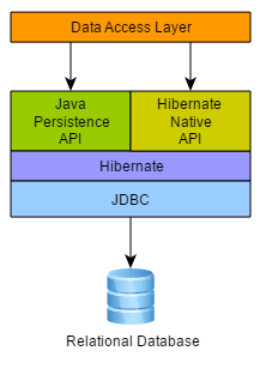
\includegraphics[width=0.4\textwidth]{hibernate.png}
\end{center}

Основные классы Hibernate такие:

\begin{itemize}
	\item Configuration --- хранит конфигурацию, в частности, к чему и как подключаться, умеет создавать SessionFactory;
	\item SessionFactory --- представляет отображение таблиц БД на классы из Data Access Layer (те самые прокси-классы), создаёт объекты Session, одна на приложение;
	\item Session --- ``Единица работы'', штука, которая реально связывается с БД и обновляет её таблицы результатами изменений в Data Access Layer;
	\item Transaction --- транзакция (атомарная операция) в БД. Сессия создаёт транзакции, но может иметь только одну открытую транзакцию в каждый момент.
\end{itemize}

Подробности суровы и многочисленны, поэтому их пока не будет. Возможно, мы вернёмся к Hibernate, когда речь пойдёт про веб-приложения (и когда мы пройдём рефлексию), пока рекомендуется страдать с JDBC (или таки самим почитать документацию по Hibernate).

\section{NoSQL, MongoDB}

Ну и конечно, ни один обзор средств работы с БД не обойдётся без упоминания NoSQL-СУБД. SQL сложный, там реляционная алгебра какая-то, а мы просто хотим хранить объекты. Так появились объектно-ориентированные СУБД, например, MongoDB. Они не умеют исполнять SQL-запросы вовсе, а хранят просто сериализованные объекты. Или, в терминологии MongoDB, \textit{документы}. Документ --- это не более чем набор пар ``ключ-значение'', при этом значение само может быть документом. Кто знает, что такое JSON, в принципе знает, про что идёт речь и тут. Документы объединены в \textit{коллекции} --- самое близкое понятие к таблице из реляционных СУБД. К коллекциям можно делать запросы в духе ``верни мне список документов, у которых такое-то поле имеет такое-то значение''. На самом деле, запросы могут быть довольно сложной комбинацией различных шаблонов, но суть примерно такая. Работает MongoDB как отдельный процесс, требует установки и запуска перед тем, как БД можно пользоваться, но обычно не требует особого администрирования --- коллекции создаются при первом обращении, никакой сложной структуры и особых метаданных в ООБД и так нет.

Пользоваться голой MongoDB из Java можно, но адово неудобно --- классы надо вручную сериализовать в JSON и писать запросы в виде строковых JSON-ов. Поэтому есть библиотека для типобезопасной работы с базой поверх mongodb-driver, которая называется Morphia. Кстати, mongodb-driver не имеет отношения к драйверам JDBC, и вообще, JDBC для ООБД не используется вовсе (что понятно, JDBC ориентирован на SQL, который ООБД не умеют).

Небольшой пример работы с MongoDB, в виде мини-туториала:

\begin{enumerate}
	\item Скачиваем и ставим сервер MongoDB: \url{https://www.mongodb.com/download-center/community}
	\item Создаём папку, где сервер будет хранить данные (по умолчанию C:/Data/db под виндой)
	\item Запускаем сервер
	\begin{itemize}
		\item start mongod.exe в консоли
		\item mongod по умолчанию лежит в C:\\Program Files\\MongoDB\\Server\\...\\bin под виндой
		\item Аналогично запускаем сервер под линуксом (\verb|mongod &|, например)
	\end{itemize}
	\item Добавляем зависимость от mongodb-driver в проект
	\begin{itemize}
		\item
			\begin{minted}{groovy}
compile 'org.mongodb:mongodb-driver-sync:3.10.1'
			\end{minted}
	\end{itemize}
	\item Добавляем зависимость ещё от Morphia (библиотека, обеспечивающая типобезопасные запросы к БД)
	\begin{itemize}
		\item
			\begin{minted}{groovy}
compile 'xyz.morphia.morphia:core:1.4.0'
			\end{minted}
	\end{itemize}
	\item Пишем класс, объекты которого будем хранить в базе:
		\begin{minted}{java}
@Entity
public class City {
    @Id
    private int id;
    private String name;

    public City() {
    }

    public City(String name) {
        this.name = name;
    }

    public String getName() {
        return name;
    }
}
		\end{minted}
	\item Код, который положит новый объект в базу:
	\begin{minted}{java}
        final Morphia morphia = new Morphia();
        morphia.mapPackage("com.example");
        final Datastore datastore = morphia.createDatastore(new MongoClient(), "mydb");

        City stPetersburg = new City("St. Petersburg");
        datastore.save(stPetersburg);
	\end{minted}
	\item Код, который зачитает объекты из базы:
	\begin{minted}{java}
        final Morphia morphia = new Morphia();
        morphia.mapPackage("com.example");
        final Datastore datastore = morphia.createDatastore(new MongoClient(), "mydb");

        for (City city : datastore.find(City.class)) {
            System.out.println(city.getName());
        }
	\end{minted}
\end{enumerate}

\end{document}
